% Options for packages loaded elsewhere
% Options for packages loaded elsewhere
\PassOptionsToPackage{unicode}{hyperref}
\PassOptionsToPackage{hyphens}{url}
\PassOptionsToPackage{dvipsnames,svgnames,x11names}{xcolor}
%
\documentclass[
  ignorenonframetext,
]{beamer}
\newif\ifbibliography
\usepackage{pgfpages}
\setbeamertemplate{caption}[numbered]
\setbeamertemplate{caption label separator}{: }
\setbeamercolor{caption name}{fg=normal text.fg}
\beamertemplatenavigationsymbolsempty
% remove section numbering
\setbeamertemplate{part page}{
  \centering
  \begin{beamercolorbox}[sep=16pt,center]{part title}
    \usebeamerfont{part title}\insertpart\par
  \end{beamercolorbox}
}
\setbeamertemplate{section page}{
  \centering
  \begin{beamercolorbox}[sep=12pt,center]{section title}
    \usebeamerfont{section title}\insertsection\par
  \end{beamercolorbox}
}
\setbeamertemplate{subsection page}{
  \centering
  \begin{beamercolorbox}[sep=8pt,center]{subsection title}
    \usebeamerfont{subsection title}\insertsubsection\par
  \end{beamercolorbox}
}
% Prevent slide breaks in the middle of a paragraph
\widowpenalties 1 10000
\raggedbottom
\AtBeginPart{
  \frame{\partpage}
}
\AtBeginSection{
  \ifbibliography
  \else
    \frame{\sectionpage}
  \fi
}
\AtBeginSubsection{
  \frame{\subsectionpage}
}
\usepackage{iftex}
\ifPDFTeX
  \usepackage[T1]{fontenc}
  \usepackage[utf8]{inputenc}
  \usepackage{textcomp} % provide euro and other symbols
\else % if luatex or xetex
  \usepackage{unicode-math} % this also loads fontspec
  \defaultfontfeatures{Scale=MatchLowercase}
  \defaultfontfeatures[\rmfamily]{Ligatures=TeX,Scale=1}
\fi
\usepackage{lmodern}

\ifPDFTeX\else
  % xetex/luatex font selection
\fi
% Use upquote if available, for straight quotes in verbatim environments
\IfFileExists{upquote.sty}{\usepackage{upquote}}{}
\IfFileExists{microtype.sty}{% use microtype if available
  \usepackage[]{microtype}
  \UseMicrotypeSet[protrusion]{basicmath} % disable protrusion for tt fonts
}{}
\makeatletter
\@ifundefined{KOMAClassName}{% if non-KOMA class
  \IfFileExists{parskip.sty}{%
    \usepackage{parskip}
  }{% else
    \setlength{\parindent}{0pt}
    \setlength{\parskip}{6pt plus 2pt minus 1pt}}
}{% if KOMA class
  \KOMAoptions{parskip=half}}
\makeatother

\usepackage{color}
\usepackage{fancyvrb}
\newcommand{\VerbBar}{|}
\newcommand{\VERB}{\Verb[commandchars=\\\{\}]}
\DefineVerbatimEnvironment{Highlighting}{Verbatim}{commandchars=\\\{\}}
% Add ',fontsize=\small' for more characters per line
\usepackage{framed}
\definecolor{shadecolor}{RGB}{241,243,245}
\newenvironment{Shaded}{\begin{snugshade}}{\end{snugshade}}
\newcommand{\AlertTok}[1]{\textcolor[rgb]{0.68,0.00,0.00}{#1}}
\newcommand{\AnnotationTok}[1]{\textcolor[rgb]{0.37,0.37,0.37}{#1}}
\newcommand{\AttributeTok}[1]{\textcolor[rgb]{0.40,0.45,0.13}{#1}}
\newcommand{\BaseNTok}[1]{\textcolor[rgb]{0.68,0.00,0.00}{#1}}
\newcommand{\BuiltInTok}[1]{\textcolor[rgb]{0.00,0.23,0.31}{#1}}
\newcommand{\CharTok}[1]{\textcolor[rgb]{0.13,0.47,0.30}{#1}}
\newcommand{\CommentTok}[1]{\textcolor[rgb]{0.37,0.37,0.37}{#1}}
\newcommand{\CommentVarTok}[1]{\textcolor[rgb]{0.37,0.37,0.37}{\textit{#1}}}
\newcommand{\ConstantTok}[1]{\textcolor[rgb]{0.56,0.35,0.01}{#1}}
\newcommand{\ControlFlowTok}[1]{\textcolor[rgb]{0.00,0.23,0.31}{\textbf{#1}}}
\newcommand{\DataTypeTok}[1]{\textcolor[rgb]{0.68,0.00,0.00}{#1}}
\newcommand{\DecValTok}[1]{\textcolor[rgb]{0.68,0.00,0.00}{#1}}
\newcommand{\DocumentationTok}[1]{\textcolor[rgb]{0.37,0.37,0.37}{\textit{#1}}}
\newcommand{\ErrorTok}[1]{\textcolor[rgb]{0.68,0.00,0.00}{#1}}
\newcommand{\ExtensionTok}[1]{\textcolor[rgb]{0.00,0.23,0.31}{#1}}
\newcommand{\FloatTok}[1]{\textcolor[rgb]{0.68,0.00,0.00}{#1}}
\newcommand{\FunctionTok}[1]{\textcolor[rgb]{0.28,0.35,0.67}{#1}}
\newcommand{\ImportTok}[1]{\textcolor[rgb]{0.00,0.46,0.62}{#1}}
\newcommand{\InformationTok}[1]{\textcolor[rgb]{0.37,0.37,0.37}{#1}}
\newcommand{\KeywordTok}[1]{\textcolor[rgb]{0.00,0.23,0.31}{\textbf{#1}}}
\newcommand{\NormalTok}[1]{\textcolor[rgb]{0.00,0.23,0.31}{#1}}
\newcommand{\OperatorTok}[1]{\textcolor[rgb]{0.37,0.37,0.37}{#1}}
\newcommand{\OtherTok}[1]{\textcolor[rgb]{0.00,0.23,0.31}{#1}}
\newcommand{\PreprocessorTok}[1]{\textcolor[rgb]{0.68,0.00,0.00}{#1}}
\newcommand{\RegionMarkerTok}[1]{\textcolor[rgb]{0.00,0.23,0.31}{#1}}
\newcommand{\SpecialCharTok}[1]{\textcolor[rgb]{0.37,0.37,0.37}{#1}}
\newcommand{\SpecialStringTok}[1]{\textcolor[rgb]{0.13,0.47,0.30}{#1}}
\newcommand{\StringTok}[1]{\textcolor[rgb]{0.13,0.47,0.30}{#1}}
\newcommand{\VariableTok}[1]{\textcolor[rgb]{0.07,0.07,0.07}{#1}}
\newcommand{\VerbatimStringTok}[1]{\textcolor[rgb]{0.13,0.47,0.30}{#1}}
\newcommand{\WarningTok}[1]{\textcolor[rgb]{0.37,0.37,0.37}{\textit{#1}}}

\usepackage{longtable,booktabs,array}
\usepackage{calc} % for calculating minipage widths
\usepackage{caption}
% Make caption package work with longtable
\makeatletter
\def\fnum@table{\tablename~\thetable}
\makeatother
\usepackage{graphicx}
\makeatletter
\newsavebox\pandoc@box
\newcommand*\pandocbounded[1]{% scales image to fit in text height/width
  \sbox\pandoc@box{#1}%
  \Gscale@div\@tempa{\textheight}{\dimexpr\ht\pandoc@box+\dp\pandoc@box\relax}%
  \Gscale@div\@tempb{\linewidth}{\wd\pandoc@box}%
  \ifdim\@tempb\p@<\@tempa\p@\let\@tempa\@tempb\fi% select the smaller of both
  \ifdim\@tempa\p@<\p@\scalebox{\@tempa}{\usebox\pandoc@box}%
  \else\usebox{\pandoc@box}%
  \fi%
}
% Set default figure placement to htbp
\def\fps@figure{htbp}
\makeatother


% definitions for citeproc citations
\NewDocumentCommand\citeproctext{}{}
\NewDocumentCommand\citeproc{mm}{%
  \begingroup\def\citeproctext{#2}\cite{#1}\endgroup}
\makeatletter
 % allow citations to break across lines
 \let\@cite@ofmt\@firstofone
 % avoid brackets around text for \cite:
 \def\@biblabel#1{}
 \def\@cite#1#2{{#1\if@tempswa , #2\fi}}
\makeatother
\newlength{\cslhangindent}
\setlength{\cslhangindent}{1.5em}
\newlength{\csllabelwidth}
\setlength{\csllabelwidth}{3em}
\newenvironment{CSLReferences}[2] % #1 hanging-indent, #2 entry-spacing
 {\begin{list}{}{%
  \setlength{\itemindent}{0pt}
  \setlength{\leftmargin}{0pt}
  \setlength{\parsep}{0pt}
  % turn on hanging indent if param 1 is 1
  \ifodd #1
   \setlength{\leftmargin}{\cslhangindent}
   \setlength{\itemindent}{-1\cslhangindent}
  \fi
  % set entry spacing
  \setlength{\itemsep}{#2\baselineskip}}}
 {\end{list}}
\usepackage{calc}
\newcommand{\CSLBlock}[1]{\hfill\break\parbox[t]{\linewidth}{\strut\ignorespaces#1\strut}}
\newcommand{\CSLLeftMargin}[1]{\parbox[t]{\csllabelwidth}{\strut#1\strut}}
\newcommand{\CSLRightInline}[1]{\parbox[t]{\linewidth - \csllabelwidth}{\strut#1\strut}}
\newcommand{\CSLIndent}[1]{\hspace{\cslhangindent}#1}



\setlength{\emergencystretch}{3em} % prevent overfull lines

\providecommand{\tightlist}{%
  \setlength{\itemsep}{0pt}\setlength{\parskip}{0pt}}



 


%% PACKAGES ---------------------------------------------------------------------------------------------------------

\usepackage{fontawesome5}
\setbeamertemplate{frametitle continuation}[from second]
\usepackage{booktabs}
\usepackage{amsmath}
\usepackage{qrcode}

%% COMMANDS ---------------------------------------------------------------------------------------------------------

% fixing the tables problem, thanks to https://github.com/quarto-dev/quarto-cli/issues/10019#issuecomment-2169284336
% \newcommand{\theHtable}{\thetable}

%% COLORS -----------------------------------------------------------------------------------------------------------

\definecolor{linkcol}{HTML}{ff46a5}
% Set all text colors to black
\setbeamercolor{normal text}{fg=black}
\setbeamercolor{frametitle}{fg=black}
\setbeamercolor{title}{fg=black}
\setbeamercolor{subtitle}{fg=black}
\setbeamercolor{author}{fg=black}
\setbeamercolor{date}{fg=black}
\setbeamercolor{block title}{fg=black}
\setbeamercolor{block body}{fg=black}

% Specific settings for section titles
\setbeamercolor{section in toc}{fg=black}    % Section titles in table of             contents
\setbeamercolor{section in head/foot}{fg=black, bg = black} % Section titles in             header/footer
\setbeamercolor{section in sidebar}{fg=black}   % Section titles in sidebar
% Use the following if section titles are displayed on separate frames:
\setbeamercolor{section in toc shaded}{fg=black}
\setbeamercolor{section title}{fg=white} 
\setbeamercolor{section in toc}{fg=black}

\setbeamertemplate{itemize item}{\color{black}$\blacktriangleright$}
\setbeamertemplate{itemize subitem}{\color{black}$\blacksquare$}
\setbeamercolor{bibliography item}{fg=black}
\setbeamercolor{bibliography entry author}{fg=black}
\setbeamercolor{bibliography entry title}{fg=black}
\setbeamercolor{bibliography entry location}{fg=black}
\setbeamercolor{bibliography entry note}{fg=black}

\setbeamercolor{enumerate item}{fg=black}
\setbeamertemplate{enumerate items}[default]
\setbeamertemplate{enumerate item}{\textbf{\color{black}\arabic{enumi}.}}

%% FONTS -----------------------------------------------------------------------------------------------------------

% Make section titles have the same size and style as frame titles
%\setbeamerfont{section title}{size=32pt,series=\bfseries} % Matches default frame title
\setbeamerfont{section title}{size={\fontsize{18}{36}}, series=\bfseries}
\setbeamerfont{frametitle}{size={\fontsize{16}{25}}, series=\mdseries}
\setbeamerfont{title}{size={\fontsize{16}{25}}, series=\bfseries}

\setbeamertemplate{section page}{
    \vfill
    {\usebeamerfont{section title}\insertsectionhead}\\
    \vfill
}

\AtBeginSection{
    \frame{\sectionpage}
}

\renewcommand{\footnotesize}{\$footnote-size$}
\makeatletter
\@ifpackageloaded{tcolorbox}{}{\usepackage[skins,breakable]{tcolorbox}}
\@ifpackageloaded{fontawesome5}{}{\usepackage{fontawesome5}}
\definecolor{quarto-callout-color}{HTML}{909090}
\definecolor{quarto-callout-note-color}{HTML}{0758E5}
\definecolor{quarto-callout-important-color}{HTML}{CC1914}
\definecolor{quarto-callout-warning-color}{HTML}{EB9113}
\definecolor{quarto-callout-tip-color}{HTML}{00A047}
\definecolor{quarto-callout-caution-color}{HTML}{FC5300}
\definecolor{quarto-callout-color-frame}{HTML}{acacac}
\definecolor{quarto-callout-note-color-frame}{HTML}{4582ec}
\definecolor{quarto-callout-important-color-frame}{HTML}{d9534f}
\definecolor{quarto-callout-warning-color-frame}{HTML}{f0ad4e}
\definecolor{quarto-callout-tip-color-frame}{HTML}{02b875}
\definecolor{quarto-callout-caution-color-frame}{HTML}{fd7e14}
\makeatother
\makeatletter
\@ifpackageloaded{caption}{}{\usepackage{caption}}
\AtBeginDocument{%
\ifdefined\contentsname
  \renewcommand*\contentsname{Table of contents}
\else
  \newcommand\contentsname{Table of contents}
\fi
\ifdefined\listfigurename
  \renewcommand*\listfigurename{List of Figures}
\else
  \newcommand\listfigurename{List of Figures}
\fi
\ifdefined\listtablename
  \renewcommand*\listtablename{List of Tables}
\else
  \newcommand\listtablename{List of Tables}
\fi
\ifdefined\figurename
  \renewcommand*\figurename{Figure}
\else
  \newcommand\figurename{Figure}
\fi
\ifdefined\tablename
  \renewcommand*\tablename{Table}
\else
  \newcommand\tablename{Table}
\fi
}
\@ifpackageloaded{float}{}{\usepackage{float}}
\floatstyle{ruled}
\@ifundefined{c@chapter}{\newfloat{codelisting}{h}{lop}}{\newfloat{codelisting}{h}{lop}[chapter]}
\floatname{codelisting}{Listing}
\newcommand*\listoflistings{\listof{codelisting}{List of Listings}}
\makeatother
\makeatletter
\makeatother
\makeatletter
\@ifpackageloaded{caption}{}{\usepackage{caption}}
\@ifpackageloaded{subcaption}{}{\usepackage{subcaption}}
\makeatother
\makeatletter
\@ifpackageloaded{sidenotes}{}{\usepackage{sidenotes}}
\@ifpackageloaded{marginnote}{}{\usepackage{marginnote}}
\makeatother
\makeatletter
\@ifpackageloaded{qrcode}{}{\usepackage{qrcode}}
\makeatother
\makeatletter
\@ifpackageloaded{fontawesome6}{}{\usepackage{fontawesome6}}
\makeatother

\usepackage{bookmark}
\IfFileExists{xurl.sty}{\usepackage{xurl}}{} % add URL line breaks if available
\urlstyle{same}
\hypersetup{
  pdftitle={Introduzione al Corso},
  pdfauthor={Filippo Gambarota PhD},
  colorlinks=true,
  linkcolor={black},
  filecolor={linkcol},
  citecolor={linkcol},
  urlcolor={linkcol},
  pdfcreator={LaTeX via pandoc}}


\title{Introduzione al Corso}
\subtitle{\textbf{ADCOM} 2025-2026}
\author{Filippo Gambarota PhD}
\date{\emph{Ultimo aggiornamento: 12-17-2025}}
\institute{Università di Padova}

\begin{document}
\frame{\titlepage}


\begin{frame}{Perchè imparare analisi dei dati?}
\phantomsection\label{perchuxe8-imparare-analisi-dei-dati}
\begin{block}{Simpson's paradox}
\phantomsection\label{simpsons-paradox}
qui esempio di california, per far vedere importanza di saper leggere e
analizzare dati

https://setosa.io/simpsons/
\end{block}

\begin{block}{La psicologia è una scienza statistica}
\phantomsection\label{la-psicologia-uxe8-una-scienza-statistica}
Rispetto al pensiero comune dove le hard-sciences (fisica, ingegneria,
matematica) richiedono competenze di analisi dei dati, sono le scienze
sociali quelle più complesse:

\begin{itemize}
\tightlist
\item
  quantità direttamente non osservabili (latenti)
\item
  grande differenze individuali scomponibile a vari livelli in
  interazione (geni-ambiente)
\item
  dinamiche complesse con molte variabili coinvolte
\end{itemize}
\end{block}

\begin{block}{Devo essere unə statisticə per fare lə psicologə?}
\phantomsection\label{devo-essere-unux259-statisticux259-per-fare-lux259-psicologux259}
Assolutamente no. Una buona metafora è:

La statistica studia il funzionamento del motore sia in termini di
funzionamento attuale che come migliorarlo. Lə scienziatə (ad esempio in
Psicologia) deve guidare bene la macchina.

Conoscere un pochino il motore aiuta MA non è necessario per essere un
buon pilota.
\end{block}

\begin{block}{Perchè capire la statistica?}
\phantomsection\label{perchuxe8-capire-la-statistica}
Tanto quanto sapere l'inglese è necessario per conoscere la letteratura
scientifica, conoscere la statistica è necessario per leggere in modo
adeguato i risultati di un paper.
\end{block}

\begin{block}{Lo dice anche il codice deontologico}
\phantomsection\label{lo-dice-anche-il-codice-deontologico}
\begin{quote}
\textbf{Articolo 5}: Lo psicologo è tenuto a mantenere un livello
adeguato di preparazione e \textbf{aggiornamento professionale}, con
particolare riguardo ai settori nei quali opera. La violazione
dell'obbligo di formazione continua, determina un illecito disciplinare
che è sanzionato sulla base di quanto stabilito dall'ordinamento
professionale. Riconosce i limiti della propria competenza e usa,
pertanto solo strumenti teorico -- pratici per i quali ha acquisito
adeguata competenza e, ove necessario, formale autorizzazione.
\textbf{Lo psicologo impiega metodologie delle quali è in grado di
indicare le fonti e riferimenti scientifici, e non suscita, nelle attese
del cliente e/o utente, aspettative infondate.}
\end{quote}
\end{block}

\begin{block}{Lo dice anche il codice deontologico}
\phantomsection\label{lo-dice-anche-il-codice-deontologico-1}
\begin{quote}
\textbf{Articolo 7}: Nelle proprie attività professionali, nelle
attività di ricerca e nelle comunicazioni dei risultati delle stesse,
nonché nelle attività didattiche, \textbf{lo psicologo valuta
attentamente, anche in relazione al contesto, il grado di validità e di
attendibilità di informazioni, dati e fonti su cui basa le conclusioni
raggiunte}; espone all'occorrenza, le ipotesi interpretative
alternative, ed esplicita i limiti dei risultati. Lo psicologo, su casi
specifici, esprime valutazioni e giudizi professionali solo se fondati
sulla conoscenza professionale diretta ovvero su una documentazione
adeguata ed attendibile.
\end{quote}
\end{block}

\begin{block}{Formule, formule, formule}
\phantomsection\label{formule-formule-formule}
Tuttə voi conoscete e capite questa formula giusto? Possiamo dare per
scontate queste cose?

\[
L(\mathbf{\beta}, \sigma^2 \mid \mathbf{y}) = \prod_{i=1}^n \frac{1}{\sqrt{2\pi \sigma^2}} \exp\left( -\frac{(y_i - \mathbf{x}_i^\top \mathbf{\beta})^2}{2\sigma^2} \right)
\]

\pause

In realtà, nemmeno io la capisco fino in fondo. L'obiettivo di questo
corso non è capire o studiare le formule ma capire più ad alto livello
quello che implicano.
\end{block}

\begin{block}{Un piccolo esempio}
\phantomsection\label{un-piccolo-esempio}
Immaginate di leggere su un paper di \textbf{due studi} dove un
\emph{gruppo clinico} e un \emph{gruppo di controllo} vengono
\textbf{confrontati} in un certo \emph{costrutto psicologico}
\textbf{misurato} tramite una certa scala self-report. Nel \textbf{primo
studio} viene raccolto un campione di 30 soggetti. Nel secondo studio
viene raccolto un campione di 300 soggetti.

\pause

Nel primo studio viene riportato che il gruppo clinico ha una misura
\emph{significativamente} maggiore nella variabile d'interesse, mentre
il secondo studio non riporta differenze \emph{significative}.

\pause

Se doveste scommettere, su quale dei due studi puntereste rispetto ad
aver trovato un risultato empiricamente \emph{vero}?
\end{block}
\end{frame}

\begin{frame}{Metodologia della ricerca}
\phantomsection\label{metodologia-della-ricerca}
https://learningstatisticswithr.com/

A theoretical construct. This is the thing that you're trying to take a
measurement of, like ``age'', ``gender'' or an ``opinion''. A
theoretical construct can't be directly observed, and often they're
actually a bit vague.

\begin{itemize}
\tightlist
\item
  A measure. The measure refers to the method or the tool that you use
  to make your observations. A question in a survey, a behavioural
  observation or a brain scan could all count as a measure.
\item
  An operationalisation. The term ``operationalisation'' refers to the
  logical connection between the measure and the theoretical construct,
  or to the process by which we try to derive a measure from a
  theoretical construct.
\item
  A variable. Finally, a new term. A variable is what we end up with
  when we apply our measure to something in the world. That is,
  variables are the actual ``data'' that we end up with in our data
  sets.
\end{itemize}
\end{frame}

\begin{frame}{Tipologia di variabili}
\phantomsection\label{tipologia-di-variabili}
\begin{block}{Diverse variabili, diverse analisi}
\phantomsection\label{diverse-variabili-diverse-analisi}
Prima di imparare ad analizzare i dati è importante capire come i dati
vengono raccolti e strutturati. Quando raccogliamo o trattiamo una
variabile, chiediamoci sempre quale sia la tipologia. Il tipo di
variabile influenza diversi aspetti, come:

\begin{itemize}
\tightlist
\item
  quali statistiche descrittive sono sensate e quali sono più
  informative
\item
  le rappresentazioni grafiche più informative
\item
  il modello statistico più adeguato per quella variabile
\end{itemize}
\end{block}

\begin{block}{Variabili, le tipologie principali}
\phantomsection\label{variabili-le-tipologie-principali}
Possiamo individuare 4 tipologie principali di variabili:

\begin{itemize}
\tightlist
\item
  \textbf{nominale}
\item
  \textbf{ordinale}
\item
  \textbf{intervalli}
\item
  \textbf{rapporti}
\end{itemize}

Questa viene anche chiamata tassonomia \textbf{NOIR}.

\marginnote{\begin{footnotesize}

Per un paper classico si veda Stevens
(\citeproc{ref-Stevens1946-te}{1946})
\href{https://stat-teaching.github.io/adcom/../materials/stevens1946.pdf}{\faIcon{file-pdf}}

\end{footnotesize}}
\end{block}

\begin{block}{Variabili di tipo \emph{nominale}}
\phantomsection\label{variabili-di-tipo-nominale}
Le variabili di tipologia \emph{nominale} sono anche definite variabili
\emph{categoriali}. Sono quindi delle etichette, verbali o numeriche,
che vengono assegnate ad una tipologia di osservazione. Ad esempio:

\begin{itemize}
\tightlist
\item
  Regione di residenza
\item
  Colore degli occhi
\item
  Religione
\item
  Categoria diagnostica
\end{itemize}

Le diverse categorie sono interscambiabili quindi \emph{non c'è un
ordine predefinito}. L'unica operazione consentita è quella di contare
le diverse categorie calcolando, in vari modi, distribuzioni di
\emph{frequenza}.
\end{block}

\begin{block}{Variabili di tipo \emph{nominale}, esempi:}
\phantomsection\label{variabili-di-tipo-nominale-esempi}
Lo vedremo meglio nelle prossime lezioni, ma possiamo rappresentare le
frequenze tramite dei \emph{barplot}:

\pandocbounded{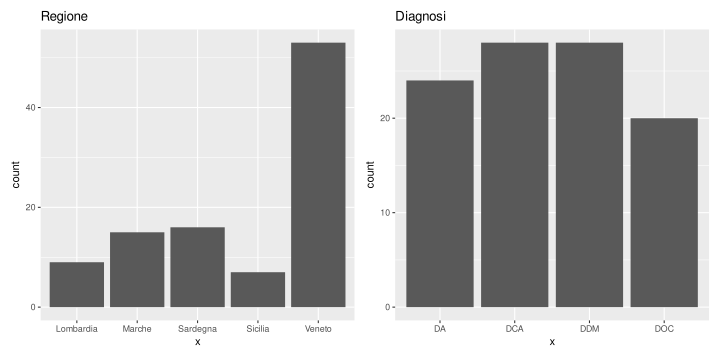
\includegraphics[keepaspectratio]{01-intro-analisi-dati_files/figure-beamer/unnamed-chunk-1-1.pdf}}
\end{block}

\begin{block}{Variabili di tipo \emph{nominale}, quali operazioni?}
\phantomsection\label{variabili-di-tipo-nominale-quali-operazioni}
\begin{tcolorbox}[enhanced jigsaw, titlerule=0mm, title=\textcolor{quarto-callout-caution-color}{\faFire}\hspace{0.5em}{Caution}, opacitybacktitle=0.6, bottomrule=.15mm, rightrule=.15mm, breakable, colframe=quarto-callout-caution-color-frame, toptitle=1mm, colback=white, coltitle=black, bottomtitle=1mm, arc=.35mm, leftrule=.75mm, opacityback=0, toprule=.15mm, left=2mm, colbacktitle=quarto-callout-caution-color!10!white]

Cosa succede, secondo voi, se dovessi calcolare la \emph{media} di una
variabile categoriale?

E se dovessi calcolare la \emph{varianza} o la \emph{mediana}?

\end{tcolorbox}

\pause

In sostanza, la tipologia di variabile è spesso legata anche a quali
operazioni sono permesse, sensate o informative. In questo caso,
calcolare la \emph{regione media} non ha alcun senso.
\end{block}

\begin{block}{Variabili di tipo \emph{ordinale}}
\phantomsection\label{variabili-di-tipo-ordinale}
Le variabili di tipo \emph{ordinale} sono quelle più comunemente
utilizzate in Psicologia ed anche quelle in un certo senso meno
intuitive.

Alcuni esempi:

\begin{itemize}
\tightlist
\item
  Risposte su scale \emph{likert}
\item
  Status socio-economico (e.g., alto, medio e basso)
\item
  Livello d'istruzione
\end{itemize}
\end{block}

\begin{block}{Variabili di tipo \emph{ordinale}}
\phantomsection\label{variabili-di-tipo-ordinale-1}
Rispetto alle variabili categoriali, le variabili \emph{ordinali} hanno
un ordine. Possiamo quindi pensarle categorie alle quali assegnamo un
numero progressivo.

\pause

Quello che non è definito per le variabili ordinali, è la
\emph{distanza} tra le categorie. Potremmo assegnare allo status
socio-economico 1 = basso, 2 = medio e 3 = alto, come 1.5, 2, 2.1.

\pause

In altri termini, la distanza tra le categorie non è nota e quindi non è
utilizzabile come informazione.
\end{block}

\begin{block}{Variabili di tipo \emph{ordinale}, esempi:}
\phantomsection\label{variabili-di-tipo-ordinale-esempi}
Anche qui, lo vedremo meglio nelle prossime lezioni ma un grafico a
barre, ordinato è un tipo di rappresentazione grafica utilizzabile.

\pandocbounded{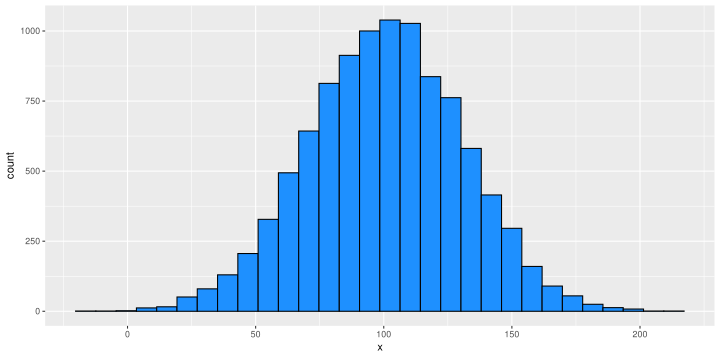
\includegraphics[keepaspectratio]{01-intro-analisi-dati_files/figure-beamer/unnamed-chunk-2-1.pdf}}
\end{block}

\begin{block}{Variabili su scala ad \emph{intervalli}}
\phantomsection\label{variabili-su-scala-ad-intervalli}
Questo è il primo tipo di variabile \emph{numerica} in senso stretto. Le
principali caratteristiche sono:

\begin{itemize}
\tightlist
\item
  L'ordine è significativo (questo viene ereditato dalle variabili
  ordinali)
\item
  Le differenze (\emph{intervalli}) tra due valori sono note e costanti
  per tutta la scala
\item
  Non c'è uno zero assoluto definito come assenza della proprietà
  misurata
\end{itemize}

La mancanza di zero assoluto rende quindi non intepretabili i rapporti
tra valori, mentre lo sono le differenze.
\end{block}

\begin{block}{Variabili su scala ad \emph{intervalli}: esempi}
\phantomsection\label{variabili-su-scala-ad-intervalli-esempi}
Alcuni esempi sono:

\begin{itemize}
\tightlist
\item
  Temperatura come ad esempio Celsius o Fahrenheit
\item
  In generale le misure psicologiche come intelligenza, personalità,
  etc.
\item
  Le date sul calendario
\end{itemize}

Possiamo dire che la distanza tra un QI di 100 e 110 è la stessa
rispetto ad un QI di 115 e 125 (sono 10 punti di QI). Non possiamo dire
che una persona che ha QI di 200 sia il doppio più intelligente di un QI
di 100.
\end{block}

\begin{block}{Variabili su scala ad \emph{intervalli}: esempi}
\phantomsection\label{variabili-su-scala-ad-intervalli-esempi-1}
\pandocbounded{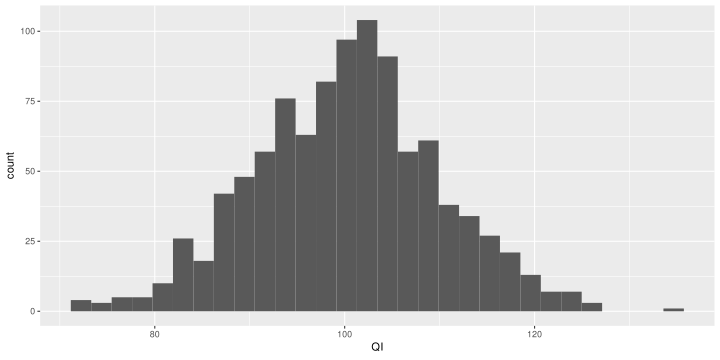
\includegraphics[keepaspectratio]{01-intro-analisi-dati_files/figure-beamer/unnamed-chunk-3-1.pdf}}
\end{block}

\begin{block}{Variabili su scala a \emph{rapporti}}
\phantomsection\label{variabili-su-scala-a-rapporti}
Questo è il tipo più completo di variabile numerica che solitamente si
trova nelle misurazioni fisiche. Eredità tutte le proprietà precedenti
aggiungendo la presenza di uno zero assoluto inteso come assenza della
proprietà.

Qualche esempio:

\begin{itemize}
\tightlist
\item
  Il tempo inteso come minuti, secondi, millisecondi: tempi di reazione
  in esperimenti cognitivi
\item
  Segnale psicofisiologico come EEG, ECG, etc.
\end{itemize}

La presenza dello zero assoluto permette di poter calcolare rapporti
significativi. Possiamo dire che 20 secondi sono il doppio del tempo
rispetto a 10 secondi.
\end{block}

\begin{block}{Tipologia di variabili, riassunto:}
\phantomsection\label{tipologia-di-variabili-riassunto}
Le 4 tipologie di variabili sono gerarchicamente ordinate rispetto alle
operazioni permissibili e significative:

\begin{itemize}
\tightlist
\item
  \emph{categoriali} --\textgreater{} uguaglianza: possiamo dire se due
  osservazioni sono nella stessa categoria
\item
  \emph{ordinali} --\textgreater{} ranking: possiamo dire chi è maggiore
  tra due osservazioni
\item
  \emph{intervalli} --\textgreater{} distanze: possiamo interpretare la
  distanza tra due osservazioni \emph{rapporti} --\textgreater{}
  rapporti: possiamo calcolare il rapporto tra due osservazioni
\end{itemize}
\end{block}

\begin{block}{Intervalli vs ordinale}
\phantomsection\label{intervalli-vs-ordinale}
Questa tassonomia non viene sempre rispettata. Ad esempio, le variabili
ordinali come le scale \emph{likert} vengono comunemente trattate come
scale ad intervalli o anche a rapporti. Ad esempio viene assunto che la
differenza tra 1 (per niente) e 2 (poco) sia la stessa che per altri
livelli.
\end{block}

\begin{block}{Operazioni permissibili}
\phantomsection\label{operazioni-permissibili}
Vedremo meglio quando parleremo delle varie statistiche descrittive.
Tuttavia, in base al tipo di variabile ci sono delle operazioni
\emph{permissibili}.

\begin{figure}[H]

{\centering \pandocbounded{\includegraphics[keepaspectratio]{img/stevens1948_table1.png}}

}

\caption{Fonte: Stevens (\citeproc{ref-Stevens1946-te}{1946})}

\end{figure}%
\end{block}
\end{frame}

\begin{frame}[fragile]{Dataset}
\phantomsection\label{dataset}
\begin{block}{Dataset}
\phantomsection\label{dataset-1}
Il \emph{dataset} è l'insieme delle variabili che sono state raccolte in
uno specifico esperimento. Contiene tutte o una parte delle variabili
che verranno utilizzate nei vari modelli statistici.

Per intenderci, possiamo immaginare un classico dataset come un foglio
Excel composto da un certo numero di righe e colonne:

\pandocbounded{\includegraphics[keepaspectratio]{img/excel-example.png}}
\end{block}

\begin{block}{Righe e colonne}
\phantomsection\label{righe-e-colonne}
Il dataset è una struttura dati \emph{bidimensionale} formata da \(n\)
righe e \(p\) colonne. La dimensione totale è \(n \times p\) (il numero
di celle). La convenzione è di indicare:

\begin{itemize}
\tightlist
\item
  \(n\) come le unità statistiche o osservazioni
\item
  \(p\) le variabili quindi le proprietà misurate su quelle specifiche
  unità statistiche
\end{itemize}

Quindi, per ogni riga \(n\) noi abbiamo tutte le caratteristiche
dell'osservazione \(n\). In ogni colonna \(p\) abbiamo tutte le
osservazioni per quella specifica caratteristica.
\end{block}

\begin{block}{Dataset come principale struttura dati}
\phantomsection\label{dataset-come-principale-struttura-dati}
Tutti i principali software per eseguire analisi dei dati come R, SPSS,
Jamovi o JASP utilizzano di base questa struttura dati bidimensionale.

Solitamente, i dati vengono raccolti tramite software ad esempio Google
Form, Qualtrics, etc. che producono in output un database, ad esempio un
foglio Excel.
\end{block}

\begin{block}{Colonne come variabili}
\phantomsection\label{colonne-come-variabili}
\textbf{Ogni colonna in un dataset è indipendente nel senso che può
essere di tipologia diversa}. Possiamo avere una colonna che indica il
nome (quindi stringhe di testo), una che indica l'età in anni (quindi
numeri interi) e una che indica il peso in kg (quindi numeri con la
virgola).

\pause

In alcuni software inoltre le variabili possono anche essere indicate
usando la tassonomia \textbf{NOIR}. Quindi possiamo avere numeri o
stringhe di testo che hanno un ordine oppure sono delle semplici
categorie.
\end{block}

\begin{block}{Colonne come variabili, Jamovi}
\phantomsection\label{colonne-come-variabili-jamovi}
\begin{figure}[H]

{\centering \pandocbounded{\includegraphics[keepaspectratio]{img/jamovi_type.png}}

}

\caption{Esempio di variabili in Jamovi}

\end{figure}%
\end{block}

\begin{block}{Colonne come variabili, R}
\phantomsection\label{colonne-come-variabili-r}
In R abbiamo diverse tipologie di dato:

\begin{Shaded}
\begin{Highlighting}[]
\FunctionTok{integer}\NormalTok{()    }\CommentTok{\# numeri interi (senza virgola)}
\FunctionTok{numeric}\NormalTok{()    }\CommentTok{\# numeri (con la virgola)}
\FunctionTok{character}\NormalTok{()  }\CommentTok{\# stringhe di testo \textasciitilde{} categoriali}
\FunctionTok{ordered}\NormalTok{()    }\CommentTok{\# stringhe di testo ordinate \textasciitilde{} ordinali}
\end{Highlighting}
\end{Shaded}
\end{block}

\begin{block}{Colonne come variabili}
\phantomsection\label{colonne-come-variabili-1}
In realtà, possiamo codificare le variabili nel modo che vogliamo, è
sufficiente avere una regola. Possiamo indicare ad esempio 4 categorie
come il colore degli occhi con i numeri da 1 a 4.

La media dei numeri da 1 a 4 è permessa ovviamente MA il risultato non
ha senso rispetto alla variabile originale.

Costruite un dataset sempre con il tipo di variabile con il tipo che più
si avvicina a quello originale, in modo da limitare questo tipo di
errori.
\end{block}

\begin{block}{Esempi di dataset}
\phantomsection\label{esempi-di-dataset}
metti qui qualche link a fogli google con esempi di dataset. Metti i
link in lettura e tu come editor.
\end{block}

\begin{block}{(cattivi) Esempi di dataset}
\phantomsection\label{cattivi-esempi-di-dataset}
qui metti qualche esempio a dataset con dei problemi:

\begin{itemize}
\tightlist
\item
  stringhe non consistenti
\item
  nessun nome di variabile
\item
  tipi delle variabili non rispettati
\end{itemize}
\end{block}
\end{frame}

\begin{frame}{La misura in Psicologia}
\phantomsection\label{la-misura-in-psicologia}
\begin{block}{La misura in Psicologia}
\phantomsection\label{la-misura-in-psicologia-1}
La misurazione in Psicologia è forse l'argomento più complesso, critico
ed affascinante di tutta la ricerca Psicologica e della Psicometria.

Lo scopo del corso non è quello di fornire una panoramica esaustiva
riguardo la misurazione ed il testing ma di fornire uno sguardo critico
rispetto alle misure che utilizziamo.

Le differenti variabili (colonne) del nostro dataset sono delle
\emph{misurazioni più o meno precise} di \emph{costrutti più o meno
definiti}.

Capire questo punto e capire come valutare la qualità delle nostre
variabili è fondamentale per comprendere i risultati dell'analisi dei
dati.
\end{block}

\begin{block}{GIGO - \textbf{G}arbage \textbf{I}n, \textbf{G}arbage
\textbf{O}ut}
\phantomsection\label{gigo---garbage-in-garbage-out}
Il GIGO è un principio cardine nell'analisi dei dati. L'idea è che non
c'è analisi sofisticata, algoritmo o procedura che possa risolvere il
problema della bassa qualità dei dati.

\pandocbounded{\includegraphics[keepaspectratio]{img/gigo.png}}
\end{block}

\begin{block}{GIGO - \textbf{G}arbage \textbf{I}n, \textbf{G}arbage
\textbf{O}ut}
\phantomsection\label{gigo---garbage-in-garbage-out-1}
In Psicologia, la qualità dei dati è sempre legata al tipo di strumento,
alla sua affidabilità, precisione e alla procedura di acquisizione.

Pensate ad un dataset dove una delle colonne identifica un punteggio ad
un questionario di depressione. Vediamo che questo è, per esempio,
maggiore in soggetti italiani vs stranieri.

Concludiamo che, per qualche motivo culturale, genetico o psicologico
gli italiani abbiano una tendenza maggiore alla depressione.
\end{block}

\begin{block}{GIGO - \textbf{G}arbage \textbf{I}n, \textbf{G}arbage
\textbf{O}ut}
\phantomsection\label{gigo---garbage-in-garbage-out-2}
Tuttavia, non abbiamo misurato la depressione come se misurassimo il
peso o l'età ma un insieme di item che \emph{in teoria} dovrebbero
essere legati al costrutto depressione.

L'assunzione implicita è quindi che:

\begin{itemize}
\tightlist
\item
  il questionario misuri effettivamente e principalmente la depressione
\item
  che misurandola più volte, questa sia più o meno simile
\item
  che gli item vengano compresi allo stesso modo
\item
  che gli item siano abbastanza sensibili da differenziare le persone
\end{itemize}
\end{block}

\begin{block}{Qualità della misura}
\phantomsection\label{qualituxe0-della-misura}
Quindi non è sufficiente avere una misura di depressione ma dobbiamo
chiederci:

\begin{itemize}
\tightlist
\item
  quanto è precisa la misura
\item
  quanto è valida e affidabile
\item
  quanto è specifica vs aspecifica
\item
  \ldots{}
\end{itemize}
\end{block}

\begin{block}{Variabili latenti e osservate}
\phantomsection\label{variabili-latenti-e-osservate}
In Psicologia, nella maggior parte dei casi siamo interessati a
costrutti detti \emph{latenti}. Latenti perchè non sono direttamente
osservabili.

Non sono direttamente osservabili ma sono indirettamente osservabili
tramite degli \emph{indicatori}. La qualità della nostra osservazione
quindi dipende dalla qualità degli indicatori.

Gli indicatori sono ad esempio gli item di un questionario o un insieme
di questionari. La variabile \emph{latente} è ad esempio la depressione.
\end{block}

\begin{block}{Un esempio}
\phantomsection\label{un-esempio}
Vediamo un esempio di item del BDI-II:

\begin{enumerate}
\setcounter{enumi}{-1}
\tightlist
\item
  Non sono più irrequieto o teso del solito.
\item
  Mi sento più irrequieto o teso del solito.
\item
  Sono così irrequieto o agitato che è difficile stare fermo.
\item
  Sono così irrequieto o agitato che devo continuare a muovermi o a fare
  qualcosa.
\end{enumerate}

Perchè questo indicatore viene utilizzato per la depressione secondo
voi?
\end{block}

\begin{block}{Un esempio}
\phantomsection\label{un-esempio-1}
Teoricamente, tra le \textbf{manifestazioni cliniche della depressione}
è presente agitazione e irrequietezza. Quindi, \textbf{se misurassi
questa manifestazione mi aspetterei, in media, punteggi elevati in
soggetti depressi}.

Quindi il collegamento tra indicatore e costrutto latente è teorico e
viene assunto o inferito dall'osservazione ma non è scontato.

Inoltre, ci possono essere molti modi diversi di misurare
l'irrequietezza che quindi concorrono a misurare (indirettamente) più o
meno accuratamente il costrutto latente.
\end{block}
\end{frame}

\begin{frame}{Validità di una misura}
\phantomsection\label{validituxe0-di-una-misura}
\begin{block}{Validità di una misura}
\phantomsection\label{validituxe0-di-una-misura-1}
La validità viene intesa come il \textbf{grado di sovrapposizione tra la
misura ed il costrutto latente}.

Spesso, semplificando, viene detto che la validità di una misura (ad
esempio un questionario) è la sua capacità di misurare quello che si
prefigge (teoricamente) di misurare.

Ci sono diversi sottotipi di validità:

\begin{itemize}
\tightlist
\item
  Validità interna
\item
  Validità esterna
\item
  Validità di costrutto
\item
  Validità di facciata
\item
  Validità ecologica
\end{itemize}
\end{block}

\begin{block}{Affidabilità di una misura}
\phantomsection\label{affidabilituxe0-di-una-misura}
La validità di una misura è la corrispondenza teorica con il costrutto
latente. L'affidabilità invece fa riferimento al processo di
misurazione.

Una misura affidabile fornisce \textbf{risultati consistenti (in base a
diversi indici) rispetto a diverse instanze del processo di misura}.

Risulta centrale quindi il concetto di \textbf{errore} di misura.
\end{block}

\begin{block}{Affidabilità, diverse tipologie}
\phantomsection\label{affidabilituxe0-diverse-tipologie}
Ci sono diverse tipologie di \emph{affidabilità} (in inglese
\emph{reliability}):

\begin{itemize}
\tightlist
\item
  Affidabilità test-retest (\emph{test-retest reliability)}
\item
  Affidabilità tra giudici (\emph{interrater realiability})
\item
  Affidabilità tra forme parallele (\emph{parallel form reliability})
\item
  Consistenza interna (\emph{internal consistency})
\end{itemize}
\end{block}

\begin{block}{Affidabilità test-retest}
\phantomsection\label{affidabilituxe0-test-retest}
Se la misura utilizzata è un indicatore di un costrutto latente
tendialmente stabile nel tempo, più misurazioni dello stesso indicatore
dovrebbero produrre risultati simili.
\end{block}

\begin{block}{Affidabilità tra giudici}
\phantomsection\label{affidabilituxe0-tra-giudici}
Se diversi giudici/sperimentatori giungono a risultati simili usando un
indicatore in modo indipendente, allora quell'indicatore ha una buona
affidabilità.
\end{block}

\begin{block}{Affidabilità tra forme parallele}
\phantomsection\label{affidabilituxe0-tra-forme-parallele}
\end{block}

\begin{block}{Consistenza interna}
\phantomsection\label{consistenza-interna}
Quando diversi indicatori sono operazionalizzazioni dello stesso
costrutto latente anche le misurazioni rilevate dovrebbero riflettere
questo legame.

In altri termini, i soggetti dovrebbero rispondere (in media) in modo
consistente ad indicatori che riflettono uno stesso costrutto latente.
\end{block}

\begin{block}{Affidabilità e validità, alcuni esempi}
\phantomsection\label{affidabilituxe0-e-validituxe0-alcuni-esempi}
Pensate a voler misurare l'ansia con un solo item chiedendo:

\begin{quote}
quanto ti senti agitatə in questo momento?
\end{quote}

Questa misura è chiaramente valida (legata teoricamente al costrutto
ansia) ma è molto instabile, poco precisa e può dipendere da molti
fattori sia personali che contestuali.

L'errore di misura dell'indicatore ansia sarebbe molto pur essendo un
indicatore teoricamente valido.
\end{block}

\begin{block}{Affidabilità e validità, alcuni esempi}
\phantomsection\label{affidabilituxe0-e-validituxe0-alcuni-esempi-1}
Un esempio invece di misure affidabili ma non per forza valide riguarda
gli indici psicofisiogici. Immaginiamo di vedere la relazione tra indici
psicofisiologici come il battito cardiaco e la depressione.

La strumentazione per misurare il battito cardiaco può essere molto
affidabile e con poco errore di misura. Tuttavia il legame tra battito
cardiaco e depressione può essere meno chiaro e non per forza del tutto
valido.
\end{block}

\begin{block}{Sensibilità e range delle misure}
\phantomsection\label{sensibilituxe0-e-range-delle-misure}
Un'altro aspetto importante riguarda la \emph{granularità} delle misure.
In altri termini, se siamo interessati a misurare variazioni nel
costrutto latente (differenza di depressione tra due gruppi di
individui) dobbiamo assicurarci che l'indicatore sia abbastanza
sensibile per cogliere queste differenze.

Sarebbe come trovare la temperatura ideale ma possiamo regolarla solo di
5 gradi alla volta. Per quanto il termostato sia affidabile e valido
come misura, la sua granularità non è adeguata.
\end{block}

\begin{block}{Effetto soffitto o pavimento}
\phantomsection\label{effetto-soffitto-o-pavimento}
In un certo senso legato alla \emph{granularità}, la mia misura deve
poter differenziare le diverse osservazioni ovvero non devono esserci
effetti \emph{soffitto} o \emph{pavimento}.

Immaginate una domanda di matematica troppo difficile o troppo facile
dove tuttə sbagliano o fanno corretto. Quella domanda non è una buona
domande perchè non mi permette di distinguere le abilità delle mie
osservazioni.
\end{block}

\begin{block}{Terminologia}
\phantomsection\label{terminologia}
Quando parliamo di esperimenti, ricerche e analisi dati la terminologia
è importante:

\begin{itemize}
\tightlist
\item
  \(y\) sono gli \textbf{outcomes} (uno o più). Solitamente chiamate
  anche \emph{variabili dipendenti} (ma preferisco \emph{outcomes})
\item
  \(x\) sono i \textbf{predittori}. Solitamente chiamate anche variabili
  \emph{indipendenti} (ma preferisco \emph{predittori})
\end{itemize}
\end{block}

\begin{block}{Terminologia}
\phantomsection\label{terminologia-1}
Per costrutto o variabile \emph{latente} intendiamo qualcosa di non
direttamente osservabile se non indirettamente tramite
\emph{indicatori}.

Il legame tra variabile latente e indicatori si chiama
\emph{operazionalizzazione} ovvero definire indicatori validi e
affidabili del costrutto latente di interesse.
\end{block}
\end{frame}

\begin{frame}{Disegni di ricerca}
\phantomsection\label{disegni-di-ricerca}
\begin{block}{Disegni di ricerca}
\phantomsection\label{disegni-di-ricerca-1}
Non tutte le ricerche dove si analizzano dei dati sono della stessa
tipologia. Le informazioni ed il grado di confidenza nel poter trarre
informazioni \emph{causali} dipende dalla tipologia di studio. Ci sono
due tipologie principali:

\begin{itemize}
\tightlist
\item
  Disegni sperimentali
\item
  Disegni non-sperimentali
\end{itemize}
\end{block}

\begin{block}{Disegni sperimentali}
\phantomsection\label{disegni-sperimentali}
Un disegno di ricerca sperimentale, ha come aspetto principale il
\emph{controllo} e la \emph{manipolazione} delle variabili, nello
specifico i predittori \(x\).

\pandocbounded{\includegraphics[keepaspectratio]{01-intro-analisi-dati_files/mediabag/img/exp-research1.pdf}}
\end{block}

\begin{block}{Disegni sperimentali, un esempio}
\phantomsection\label{disegni-sperimentali-un-esempio}
Il classico esempio è la ricerca medica. Voglio valutare l'efficiacia di
un certo farmaco o trattamento (\(x\)). Semplificando somministro il
trattamento sul 50\% dei soggetti e un placebo nel restante 50\%.

Se l'outcome \(y\) cambia tra i due gruppi, c'è una relazione causale
tra il trattamento \(x\) ed il cambiamento nell'outcome \(y\).
\end{block}

\begin{block}{Disegni sperimentali}
\phantomsection\label{disegni-sperimentali-1}
Questo presuppone che, i due gruppi differiscano solo per il trattamento
\(x\) e tutte le altre variabili (che potrebbero avere un effetto) siano
\emph{controllate}.

Questo non è sempre (mai) possibile e quindi si ricorre alla
\emph{randomizzazione}. Assegnando casualmente i soggetti ai due gruppi
si limita l'impatto di altre variabili.
\end{block}

\begin{block}{Randomizzazione, perchè funziona?}
\phantomsection\label{randomizzazione-perchuxe8-funziona}
Immaginate di avere 100 persone, un trattamento \(x\) ed un outcome
\(y\). Immaginate che per qualche ragione, l'età (per semplicità adulti
e anziani) sia associata ad un diverso livello di \(y\).

\pandocbounded{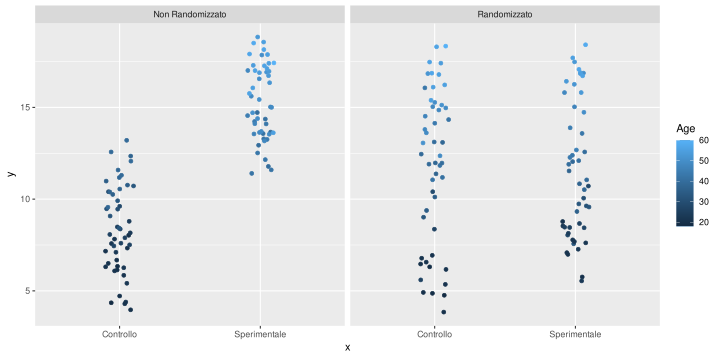
\includegraphics[keepaspectratio]{01-intro-analisi-dati_files/figure-beamer/unnamed-chunk-5-1.pdf}}
\end{block}

\begin{block}{Randomizzazione, perchè funziona?}
\phantomsection\label{randomizzazione-perchuxe8-funziona-1}
La \emph{randomizzazione} quindi mitiga (e in teoria rimuove) l'effetto
di variabili non direttamente controllate assegnando gli individui in
modo casuale al trattamento.
\end{block}

\begin{block}{Perchè non randomizziamo sempre?}
\phantomsection\label{perchuxe8-non-randomizziamo-sempre}
Il non randomizzare non è una scelta spesso. Ci sono delle condizioni
dove non è possibile randomizzare per motivi etici o strettamente
empirici.

Immaginate di dover capire l'impatto sulla salute di un certo
comportamento (e.g., mangiare un certo alimento). Idealmente dovreste
prendere in modo casuale soggetti, assegnarli una dieta e vedere
l'impatto.

Quello che invece si fa è raccogliere su larga scala le abitudini di un
campione di soggetti e vedere le \emph{associazioni} con l'outcome.
\end{block}

\begin{block}{Perchè non randomizziamo sempre?}
\phantomsection\label{perchuxe8-non-randomizziamo-sempre-1}
Il problema è che non potendo randomizzare, non è possibile isolare
chiaramente l'effetto del predittore d'interesse.

In realtà possiamo:

\begin{itemize}
\tightlist
\item
  Includere tutte le possibili variabili come predittore
  (\emph{regressione multipla}) ma questo è valido solo se siamo sicuri
  di averle inserite tutte (molto poco plausibile)
\item
  Evidenziare un'associazione tra \(x\) e \(y\) ma senza poterne trarre
  una relazione causale.
\end{itemize}
\end{block}

\begin{block}{Quasi-esperimenti}
\phantomsection\label{quasi-esperimenti}
I quasi-esperimenti o studi osservazionali sono quelli studi dove
vengono rilevate delle variabli e si vedono le associazioni.

Consegnare un questionario a \(n\) persone e vedere associazioni tra
variabili è uno studio osservazionale dove quasi mai possiamo inferire
relazioni causali.
\end{block}

\begin{block}{Disegni di ricerca}
\phantomsection\label{disegni-di-ricerca-2}
Mellis (\citeproc{ref-Mellis2020-py}{2020}) fornisce una panoramica
sulla tipologia di studi. Anche questo sito
\url{https://www.cebm.ox.ac.uk/resources/ebm-tools/study-designs}
fornisce una rappresentazione grafica. La nomenclatura dipende molto
dalla disciplina ma la grande distinzione è la presenza o meno di
randomizzazione e la manipolazione delle variabili.

\pandocbounded{\includegraphics[keepaspectratio]{img/study-design.jpg}}
\end{block}
\end{frame}

\begin{frame}{Confounder e artefatti}
\phantomsection\label{confounder-e-artefatti}
\begin{block}{Confounder e artefatti}
\phantomsection\label{confounder-e-artefatti-1}
La validità di uno studio e di un'analisi dei dati può essere
compromessa da \emph{confounder} e \emph{artefatti}. I confounder, come
dice la parola, sono variabili che confondono la relazione che assumiamo
e osserviamo tra \(x\) e \(y\).

\pandocbounded{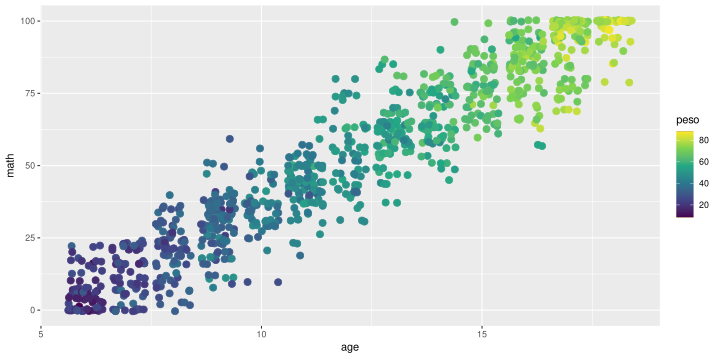
\includegraphics[keepaspectratio]{01-intro-analisi-dati_files/figure-beamer/unnamed-chunk-6-1.pdf}}
\end{block}

\begin{block}{Confounder}
\phantomsection\label{confounder}
L'idea è che se c'è una variabile \(z\) che è legata sia ad \(x\) che a
\(y\) ma io non la osservo/raccolgo. La relazione tra \(x\) e \(y\) è
parzialmente o totalmente spuria.
\end{block}

\begin{block}{Confounder, un esempio}
\phantomsection\label{confounder-un-esempio}
Immaginate di raccogliere dei dati di bambinə e ragazzə dai 6 ai 18
anni. Raccogliete punteggi a test di matematica e raccogliete il peso.
Non avete altre informazioni.

\qrcode[]{https://docs.google.com/spreadsheets/d/16JRt1_tXYQntv2bcbvbqoOzPEZvcXPKFYpvolR16c5E/edit?gid=0#gid=0}
    

Andate a questo link e provate ad esplorare il dataset. Quali potrebbero
essere dei confounder?
\end{block}

\begin{block}{Confounder, un esempio}
\phantomsection\label{confounder-un-esempio-1}
In pratica, \(z\) (l'età in questo caso) è una variabile legata sia a
\(x\) che a \(y\) che non osserviamo ma spiega totalmente (o
parzialmente) la relazione \(y \sim x\). Vedremo come tenere conto di
\(z\) statisticamente ma i confounder possono renderci la vita molto
complessa.

\pandocbounded{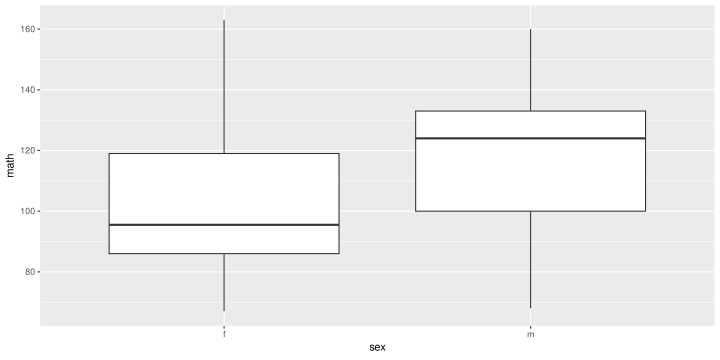
\includegraphics[keepaspectratio]{01-intro-analisi-dati_files/figure-beamer/unnamed-chunk-7-1.pdf}}
\end{block}

\begin{block}{Simpson's Paradox}
\phantomsection\label{simpsons-paradox-1}
Nell'autunno del 1973, l'Università della California a Berkeley rese
pubblici i dati relativi alle ammissioni ai corsi di laurea magistrale.
I dati riportavano il corso (dipartimento) per cui il candidato aveva
fatto domanda, il genere auto-dichiarato (Maschio o Femmina) e se la
domanda era stata accettata o respinta.

\pandocbounded{\includegraphics[keepaspectratio]{01-intro-analisi-dati_files/figure-beamer/unnamed-chunk-8-1.pdf}}

\marginnote{\begin{footnotesize}

Si veda Bickel et al. (\citeproc{ref-Bickel1975-or}{1975})

\end{footnotesize}}
\end{block}

\begin{block}{Riferimenti}
\phantomsection\label{riferimenti}
\phantomsection\label{refs}
\begin{CSLReferences}{1}{0}
\bibitem[\citeproctext]{ref-Bickel1975-or}
Bickel, P. J., Hammel, E. A., \& O'connell, J. W. (1975). {Sex bias in
graduate admissions: data from berkeley: Measuring bias is harder than
is usually assumed, and the evidence is sometimes contrary to
expectation}. \emph{Science (New York, N.Y.)}, \emph{187}, 398--404.
\url{https://doi.org/10.1126/science.187.4175.398}

\bibitem[\citeproctext]{ref-Mellis2020-py}
Mellis, C. M. (2020). {How to choose your study design}. \emph{Journal
of Paediatrics and Child Health}, \emph{56}, 1018--1022.
\url{https://doi.org/10.1111/jpc.14929}

\bibitem[\citeproctext]{ref-Stevens1946-te}
Stevens, S. S. (1946). {On the theory of scales of measurement}.
\emph{Science (New York, N.Y.)}, \emph{103}, 677--680.
\url{https://doi.org/10.1126/science.103.2684.677}

\end{CSLReferences}
\end{block}
\end{frame}




\end{document}
